\documentclass[aspectratio=169]{beamer}
\usepackage{etex} % fixes new-dimension error
\usepackage{lmodern}
\usepackage[T1]{fontenc}

\usepackage{graphicx,amsmath}
\usepackage{stmaryrd} % cf. interleave
\usepackage{booktabs}
\usepackage{amscd}
\usepackage{multicol}
\usepackage[absolute,overlay]{textpos}
\usepackage{alltt}
\usepackage{proof}
\usepackage{subcaption}
\usepackage{tikz}
\usepackage{tikz-cd}
\usepackage[new]{old-arrows}
\usepackage[all]{xy}
\usepackage{pgfplots}
\usepackage{textcomp}

\renewcommand\familydefault{\sfdefault}
 
%input preamble and macros
% \input{../slides/macros/preamble}
\usepackage{etex} % fixes new-dimension error
\usepackage{lmodern}
\usepackage[T1]{fontenc}

%----------------------------------------------------------------------------
\usepackage{graphicx,amsmath}
\usepackage{stmaryrd} % cf. interleave
\usepackage{booktabs}
\usepackage{amscd}
\usepackage{multicol}
\usepackage[absolute,overlay]{textpos}
\usepackage{alltt}
\usepackage{proof}
\usepackage{subcaption}
\usepackage{tikz}
\usepackage{tikz-cd}
\usepackage[new]{old-arrows}
\usepackage[all]{xy}
\usepackage{pgfplots}
\usepackage{textcomp}


\usepackage{transparent}
\usepackage{xspace}
\usepackage{listings}
\usepackage{pdfpages}
\usepackage{relsize}

%%%%%%%%%%%%% Macros
\newcommand{\Ban}{\catfont{Ban}}
\newcommand{\Met}{\catfont{Met}}
\newcommand{\Shuff}{\mathrm{Sf}}
\newcommand{\Cats}{\catfont{Cat}}
\newcommand{\VCat}{\mathcal{V}\text{-}\Cats}
\newcommand{\VCatSy}{\mathcal{V}\text{-}\Cats_{\mathsf{sym}}}
\newcommand{\VCatSe}{\mathcal{V}\text{-}\Cats_{\mathsf{sep}}}
\newcommand{\VCatSS}{\mathcal{V}\text{-}\Cats_{\mathsf{sym,sep}}}
%%%% Categories
\newcommand{\catfont}[1]{\mathsf{#1}}
\newcommand{\cop}{\catfont{op}}
\newcommand{\Law}{\catfont{Law}}
\newcommand{\catV}{\catfont{V}}
\newcommand{\catX}{\catfont{X}}
\newcommand{\catC}{\catfont{C}}
\newcommand{\catD}{\catfont{D}}
\newcommand{\catA}{\catfont{A}}
\newcommand{\catB}{\catfont{B}}
\newcommand{\catI}{\catfont{I}}
\newcommand{\Set}{\catfont{Set}}
\newcommand{\Top}{\catfont{Top}}
\newcommand{\Pos}{\catfont{Pos}}
\newcommand{\Inj}{\catfont{Inj}}
\newcommand{\Det}{\catfont{RMhat}}
\newcommand{\CoAlg}[1]{\catfont{CoAlg}\left (#1 \right )}
\newcommand{\Mon}{\catfont{Mon}}
\newcommand{\Mnd}{\catfont{Mnd}(\catC)}
\newcommand{\SMnd}{\catfont{Mnd}(\Set)}
\newcommand{\CLat}{\catfont{CLat}}
\newcommand{\Stone}{\catfont{Stone}}
\newcommand{\Spectral}{\catfont{Spectral}}
\newcommand{\CompHaus}{\catfont{CompHaus}}
\newcommand{\Subs}[2]{\catfont{Sub}_{}}
\newcommand{\Cone}{\catfont{Cone}}
\newcommand{\StComp}{\catfont{StablyComp}}
\newcommand{\PosC}{\catfont{PosComp}}
\newcommand{\Haus}{\catfont{Haus}}
\newcommand{\Meas}{\catfont{Meas}}
\newcommand{\Ord}{\catfont{Ord}}
\newcommand{\EndoC}{[\catC,\catC]}
%% General functors
\newcommand{\funfont}[1]{#1}
\newcommand{\funF}{\funfont{F}}
\newcommand{\funU}{\funfont{U}}
\newcommand{\funG}{\funfont{G}}
\newcommand{\funT}{\funfont{T}}
\newcommand{\funI}{\funfont{I}}
%% Particular kinds of functors
\newcommand{\sfunfont}[1]{\mathrm{#1}}
\newcommand{\Pow}{\sfunfont{P}}
\newcommand{\Dist}{\sfunfont{D}}
\newcommand{\Maybe}{\sfunfont{M}}
\newcommand{\List}{\sfunfont{L}}
\newcommand{\UForg}{\sfunfont{U}}
\newcommand{\Forg}[1]{\sfunfont{U}_{#1}}
\newcommand{\Id}{\sfunfont{Id}}
\newcommand{\Vie}{\sfunfont{V}}
\newcommand{\Disc}{\funfont{D}}
\newcommand{\Weight}{\sfunfont{W}}
\newcommand{\homf}{\sfunfont{hom}}
\newcommand{\Yoneda}{\sfunfont{Y}}
%% Diagram functors
\newcommand{\Diag}{\mathscr{D}}
\newcommand{\KDiag}{\mathscr{K}}
\newcommand{\LDiag}{\mathscr{L}}
%% Monads
\newcommand{\monadfont}[1]{\mathbb{#1}}
\newcommand{\monadT}{\monadfont{T}}
\newcommand{\monadS}{\monadfont{S}}
\newcommand{\monadU}{\monadfont{U}}
\newcommand{\monadH}{\monadfont{H}}
\newcommand{\str}{\mathrm{str}}
%% Adjunctions
\newcommand\adjunct[2]{\xymatrix@=8ex{\ar@{}[r]|{\top}\ar@<1mm>@/^2mm/[r]^{{#2}}
& \ar@<1mm>@/^2mm/[l]^{{#1}}}}
\newcommand\adjunctop[2]{\xymatrix@=8ex{\ar@{}[r]|{\bot}\ar@<1mm>@/^2mm/[r]^{{#2}}
& \ar@<1mm>@/^2mm/[l]^{{#1}}}}
%% Retractions
\newcommand\retract[2]{\xymatrix@=8ex{\ar@{}[r]|{}\ar@<1mm>@/^2mm/@{^{(}->}[r]^{{#2}}
& \ar@<1mm>@/^2mm/@{->>}[l]^{{#1}}}}
%% Limits
\newcommand{\pv}[2]{\langle #1, #2 \rangle}
\newcommand{\limt}{\mathrm{lim}}
\newcommand{\pullbackcorner}[1][dr]{\save*!/#1+1.2pc/#1:(1,-1)@^{|-}\restore}
\newcommand{\pushoutcorner}[1][dr]{\save*!/#1-1.2pc/#1:(-1,1)@^{|-}\restore}
%% Colimits
\newcommand{\colim}{\mathrm{colim}}
\newcommand{\inl}{\mathrm{inl}}
\newcommand{\inr}{\mathrm{inr}}
%% Distributive categories
\newcommand{\distr}{\mathrm{dist}}
\newcommand{\undistr}{\mathrm{undist}}
%% Closedness
\newcommand{\curry}[1]{\mathrm{curry}{#1}}
\newcommand{\app}{\mathrm{app}}
%% Misc. operations
\newcommand{\const}[1]{\underline{#1}}
\newcommand{\comp}{\cdot}
\newcommand{\id}{\mathrm{id}}
%% Factorisations
\newcommand{\EClass}{E}
\newcommand{\MClass}{M}
\newcommand{\MConeClass}{\mathcal{M}}
%%%%%%%%%%%%%%%% End of Categorical Stuff

%%%% Misc
%% Operations
\newcommand{\blank}{\, - \,}
\newcommand{\sem}[1]{\llbracket #1 \rrbracket}
\newcommand{\closure}[1]{\overline{#1}}
% \DeclareMathOperator{\img}{\mathrm{im}}
% \DeclareMathOperator{\dom}{\mathrm{dom}}
% \DeclareMathOperator{\codom}{\mathrm{codom}}
%% Sets of numbers
\newcommand{\N}{\mathbb{N}}
\newcommand{\Z}{\mathbb{Z}}
\newcommand{\Nats}{\mathbb{N}}
\newcommand{\Reals}{\mathbb{R}}
\newcommand{\Rz}{\Reals_{\geq 0}}
\newcommand{\Complex}{\mathbb{C}}
%% Writing
\newcommand{\cf}{\emph{cf.}}
\newcommand{\ie}{\emph{i.e.}}
\newcommand{\eg}{\emph{e.g.}}
\newcommand{\df}[1]{\emph{\textbf{#1}}}
%%%%%%%%%%%%%%%% End of Misc

%%%% Programming Stuff
%% Types
\newcommand{\typefont}[1]{\mathbb{#1}}
\newcommand{\typeOne}{1}
\newcommand{\typeTwo}{2}
\newcommand{\typeA}{\typefont{A}}
\newcommand{\typeX}{\typefont{X}}
\newcommand{\typeB}{\typefont{B}}
\newcommand{\typeC}{\typefont{C}}
\newcommand{\typeV}{\typefont{V}}
\newcommand{\typeD}{\typefont{D}}
\newcommand{\typeI}{\typefont{I}}
%% RuleName
\newcommand{\rulename}[1]{(\mathrm{#1})}
%% Sequents
\newcommand{\jud}{\vdash}
\newcommand{\vljud}{\rhd}
\newcommand{\cojud}{\vdash_{\co}}
\newcommand{\vl}{\mathtt{v}}
\newcommand{\co}{\mathtt{c}}
% Program font
\newcommand{\prog}[1]{\mathtt{#1}}
\newcommand{\pseq}[3]{#1 \leftarrow #2; #3}
\newcommand{\ppm}[4]{(#1,#2) \leftarrow #3; #4}
\newcommand{\pinl}[1]{\prog{inl}(#1)}
\newcommand{\pinr}[1]{\prog{inr}(#1)}
\newcommand{\pcase}[4]{\prog{ case } #1 \prog{ of } \pinl{#2} \Rightarrow #3 ; \pinr{#2} \Rightarrow #4}
%% Sets of terms
\newcommand{\ValuesBP}[2]{\mathsf{Values}(#1, #2)}
\newcommand{\TermsBP}[2]{\mathsf{Terms}(#1, #2)}
\newcommand{\closValP}[1]{\ValuesBP{\emptyset}{#1}}
\newcommand{\closTermP}[1]{\TermsBP{\emptyset}{#1}}
\newcommand{\closVal}{\closValP{\typeA}}
\newcommand{\closTerm}{\closTermP{\typeA}}
%% Contextual equivalence
\newcommand{\ctxeq}{\equiv_{\prog{ctx}}}
%%%% End of Programming Stuff

%------ Setting lecture info ----------------------------------------------
\newcounter{lectureID}
\stepcounter{lectureID}
\newcommand{\getLecture}{\arabic{lectureID}\xspace}
\newcommand{\setLectureBasic}[1]{
  \title{
    #1
    }
  \author{Jos\'{e} Proen\c{c}a}
  \institute{CISTER -- U.Porto, Porto, Portugal
            \hfill 
            \begin{tabular}{r@{}}
            \url{https://fm-dcc.github.io/sv2425}
            \end{tabular}
            }
  \date{System Verification (CC4084) 2024/2025}
  % logos of institutions
  \titlegraphic{
    \begin{textblock*}{5cm}(4.0cm,6.80cm)
       
\includegraphics[scale=0.18]{images/fcup}\hspace*{.85cm}~%
    \end{textblock*}
    \begin{textblock*}{5cm}(8.4cm,7.25cm)
      % \includegraphics[scale=0.50]{images/dcc}
      
\includegraphics[scale=0.20]{images/cister}
    \end{textblock*}
  }  
}
\newcommand{\setLecture}[2]{\setcounter{lectureID}{#1}\setLectureBasic{#1. #2}}

%------ Counters for exercises ----------------------------------------------
\newcounter{cExercise}
\newcommand{\exercise}{\stepcounter{cExercise}Ex.\,\arabic{lectureID}.\arabic{cExercise}:\xspace}
\newcommand{\exerciseBack}{\addtocounter{cExercise}{-1}}
\newcommand{\exerciseAdd}{\stepcounter{cExercise}}
\newcommand{\doExercise}[3][0mm]{\begin{exampleblock}{\exercise #2}\wrap{\rule{0pt}{#1}}#3\end{exampleblock}}
\newcommand{\doSimpleExercise}[2][0mm]{\begin{exampleblock}{}\wrap{\rule{0pt}{#1}}\structure{\textbf{\exercise} #2}\end{exampleblock}}

% Slide
\newenvironment{slide}[1]{\begin{frame}\frametitle{#1}}{\end{frame}}

% Misc by José
\newcommand{\wrap}[2][]{\begin{tabular}[#1]{@{}c@{}}#2\end{tabular}}
\newcommand{\mwrap}[1]{\ensuremath{\begin{array}{@{}c@{}}#1\end{array}}}
\def\trans#1{\xrightarrow{#1}}  % - a - > 
\def\Trans#1{\stackrel{#1}{\Longrightarrow}} % =a=> 
\newcommand{\transp}[2][35]{\color{fg!#1}#2}
\newcommand{\transpt}[2][.35]{\tikz{\node[inner sep=1pt,fill opacity=0.5]{#2}}}
\newcommand{\faded}[2][0.4]{{\transparent{#1}#2}} % alternative to "transp" using transparent package
\newcommand{\set}[1]{\left\{ #1 \right\}} % {a,b,...z}
\newcommand{\mi}[1]{\ensuremath{\mathit{#1}}\xspace}
\newcommand{\mf}[1]{\ensuremath{\mathsf{#1}}\xspace}
% \newcommand{\gold}[1]{\textcolor{darkgoldenrod}{#1}\xspace}


%------ using color ---------------------------------------------------------
\definecolor{goldenrod}{rgb}{.80392 .60784 .11373}
\definecolor{darkgoldenrod}{rgb}{.5451 .39608 .03137}
\definecolor{brown}{rgb}{.15 .15 .15}
\definecolor{darkolivegreen}{rgb}{.33333 .41961 .18431}
\definecolor{myGray}{gray}{0.85}
%
%
\newcommand{\red}[1]{\textcolor{red!80!black}{#1}\xspace}
\newcommand{\blue}[1]{\textcolor{blue}{#1}\xspace}
\newcommand{\gold}[1]{\textcolor{darkgoldenrod}{#1}\xspace}
\newcommand{\gray}[1]{\textcolor{myGray}{#1}\xspace}
% \def\alert#1{{\darkgoldenrod #1}}
% \def\alert#1{{\alert{#1}}}
%\def\brw#1{{\brown #1}}
% \def\structure#1{{\blue #1}}
% \def\tstructure#1{\textbf{\darkblue #1}}
%%\def\gre#1{{\green #1}}
\def\gre#1{{\darkolivegreen #1}}
\def\gry#1{{\textcolor{gray}{#1}}}
\def\rdb#1{{\red #1}}
\def\st{\mathbf{.}\,}
\def\laplace#1#2{*\txt{\mbox{ \fcolorbox{black}{myGray}{$\begin{array}{c}\mbox{#1}\\\\#2\\\\\end{array}$} }}}
%\newcommand{\galois}[2]{#1\; \dashv\; #2}



% ----- from LSB
\def\Act{N}
\def\cnil{\mathbf{0}}
\def\cpf#1#2{#1 . #2}                           % a.P
\def\cou#1#2{#1 \mathbin{+} #2}                 % P + Q
%\def\crt#1#2{\mathbin{#1 \setminus_{#2}}}       % P \ A
%\def\crtt#1#2{\mathbin{#1 \setminus\!\setminus_{#2}}}       % P \ A
%\def\crt#1#2{\mathsf{new}\, #2\;  #1}       % P \ A
\def\crt#1#2{#1 \backslash #2}       % P \ A
%\def\crn#1#2{\{#2\}\, #1}                  % P[f]
\def\ainv#1{\overline{#1}}
\def\rtran#1{\stackrel{#1}{\longrightarrow}}
% \def\pair#1{\const{#1}}
\def\pair#1{\langle #1 \rangle}
\def\asor{\mathbin{|}}                    % A | B
\def\setdef#1#2{\mathopen{\{} #1 \asor #2 \mathclose{\}}}
\def\imp{\mathbin{\Rightarrow}}
\def\dimp{\mathbin{\Leftrightarrow}}
\def\rimp{\mathbin{\Leftarrow}}
\def\rra{\longrightarrow}
\def\rcb#1#2#3#4{\def\nothing{}\def\range{#3}\mathopen{\langle}#1 \ #2 \ \ifx\range\nothing::\else: \ #3 :\fi \ #4\mathclose{\rangle}}
\def\aconv#1{#1^{\circ}} 
\def\abv{\stackrel{\rm abv}{=}}


\def\crn#1#2{\mathbin{#1[#2]}}                  % P[f]
\def\couit#1#2{\Sigma_{#1}#2}                  %  + i=1,n
\def\cpar#1#2{#1 \mid #2}                       %  |
\def\ctpar#1#2{#1 \parallel #2}                       %  |
\def\cpars#1#2#3{#1 \mid_{#3} #2}               %  |S

% Spliting frames in 2 columns
\newcommand{\splittwo}[4]{ 
  \begin{columns}[T]% align columns
  \begin{column}{#1\textwidth} #3 \end{column} ~~~
  \begin{column}{#2\textwidth} #4 \end{column} \end{columns}
}
\newcommand{\frsplit}[3][.48]{
  \begin{columns}%[T] % align columns
  \begin{column}{#1\textwidth} #2 \end{column} ~~~
  \begin{column}{#1\textwidth} #3 \end{column} \end{columns}
}
\newcommand{\frsplitdiff}[5][]{
  \begin{columns}[#1]%[T] % align columns
  \begin{column}{#2\textwidth} #4 \end{column} ~~~
  \begin{column}{#3\textwidth} #5 \end{column} \end{columns}
}
\newcommand{\frsplitt}[3][.48]{
  \begin{columns}[T] % align columns
  \begin{column}{#1\textwidth} #2 \end{column} ~~~
  \begin{column}{#1\textwidth} #3 \end{column} \end{columns}
}
\newcommand{\col}[2][.48]{\begin{column}{#1\textwidth} #2 \end{column}}
\newcommand{\colb}[3][.48]{\begin{column}{#1\textwidth} \begin{block}{#2} #3 \end{block} \end{column}}

% Spliting frames in 3 columns
\newcommand{\splitthree}[6]{
  \begin{columns}[T] % align columns
  \begin{column}{#1\textwidth} #4 \end{column} ~~~
  \begin{column}{#2\textwidth} #5 \end{column} ~~~
  \begin{column}{#3\textwidth} #6 \end{column} \end{columns}
}
\newcommand{\frsplitthree}[4][.31]{
  \begin{columns}%[T] % align columns
  \begin{column}{#1\textwidth} #2 \end{column} ~~~
  \begin{column}{#1\textwidth} #3 \end{column} ~~~
  \begin{column}{#1\textwidth} #4 \end{column} \end{columns}
}
\newcommand{\frsplitdiffthree}[5]{
  \begin{columns}%[T] % align columns
  \begin{column}{#1\textwidth} #3 \end{column} ~~~
  \begin{column}{#1\textwidth} #4 \end{column} ~~~
  \begin{column}{#2\textwidth} #5 \end{column} \end{columns}
}
\newcommand{\frsplittthree}[4][.32]{
  \begin{columns}[T] % align columns
  \begin{column}{#1\textwidth} #2 \end{column} ~
  \begin{column}{#1\textwidth} #3 \end{column} ~
  \begin{column}{#1\textwidth} #4 \end{column} \end{columns}
}


\newcommand{\typerule}[4][]{\ensuremath{\begin{array}[#1]{c}\textsf{\scriptsize ({#2})} \\#3 \\\hline\raisebox{-3pt}{\ensuremath{#4}}\end{array}}}
\newcommand{\styperule}[3][]{\ensuremath{\begin{array}[#1]{c} #2 \\[0.5mm]\hline\raisebox{-4pt}{\ensuremath{#3}}\end{array}}}
\newcommand{\shrk}{\vspace{-3mm}}

\def\caixa#1{\medskip
  \begin{center}
  \fbox{\begin{minipage}{0.9\textwidth}\protect{#1}\end{minipage}}
  \end{center}}

% \newcommand{\mybox}[2][0.9]{
%   \begin{minipage}{#1\textwidth}\begin{block}{}\centering #2\end{block}\end{minipage}}
% \newcommand{\mycbox}[2][0.9]{
%   {\\[-5mm]\centering\mybox[#1]{#2}\\[-5mm]}}
\newcommand{\mybox}[2][4mm]{
  % \begin{minipage}{#1\textwidth}\begin{block}{}\centering #2\end{block}\end{minipage}}
  \tikz{\node[fill=barcolor!40,align=center,inner sep=#1]{#2};}}
\newcommand{\mycbox}[2][4mm]{
  \begin{center}\mybox[#1]{#2}\end{center}}
  % {\\[-5mm]\centering\mybox[#1]{#2}\\[-5mm]}}



%%%%% Tikz
% \usetikzlibrary{arrows.meta, calc, fit, tikzmark}
\usetikzlibrary{%
  positioning
 ,patterns
 ,arrows
 ,arrows.meta
 ,automata
 ,calc
 ,shapes
 ,fit
 ,tikzmark
 ,fadings
 ,decorations.pathreplacing
 ,plotmarks
% ,pgfplots.groupplots
 ,decorations.markings
 ,shadows
}
% \tikzset{shorten >=1pt,node distance=2cm,on grid,auto,initial text={},inner sep=2pt}
\tikzstyle{aut}=[shorten >=1pt,node distance=2cm,on grid,auto,initial text={},inner sep=2pt]
\tikzstyle{st}=[circle,draw=black,fill=black!10,inner sep=3pt]
\tikzstyle{sst}=[rectangle,draw=none,fill=none,inner sep=3pt]
\tikzstyle{final}=[accepting]
\tikzstyle{lbl}=[font=\footnotesize,inner sep=3pt]

% For modal logic and timed automata slides
\def\uppaal{\textsc{Uppaal}}
\def\cc#1{\mathcal{C}(#1)}
% % \newcommand{\pv}[2]{\langle #1 \rangle\, #2}
% \newcommand{\nc}[2]{[#1]\, #2}
\newcommand{\impp}{\mathbin{\rightarrow}}
\newcommand{\dimpp}{\mathbin{\leftrightarrow}}
\newcommand{\always}{\boxempty}
\newcommand{\nexts}{\bigcirc}
\newcommand{\until}{\mathbin{\mathcal U}}
\newcommand{\eventual}{\Diamond}
\newcommand{\true}{\mathsf{true}}
\newcommand{\false}{\mathsf{false}}
\newcommand{\fdec}[3]{#1: #2 \longrightarrow  #3}
\newcommand{\pow}[1]{{\cal P}#1}
\newcommand{\tran}[1]{\stackrel{#1}{\longrightarrow}}
\newcommand{\PP}{\alert{P}}
\newcommand{\universal}[2]{\forall_{#1}\; .\; #2}
\newcommand{\existential}[2]{\exists_{#1}\; .\; #2}
\newcommand{\enset}[1]{\mathopen{ \{ }#1\mathclose{ \} }} % {a,b,...z}
\newcommand{\diam}[1]{\ensuremath{\langle #1 \rangle}}
\newcommand{\boxx}[1]{\ensuremath{[#1]}}
\newcommand{\evm}[1]{\langle #1 \rangle\,}
\newcommand{\alm}[1]{[#1]\,}
\newcommand{\evmb}[1]{\evm{\alert{#1}}}
\newcommand{\almb}[1]{\alm{\alert{#1}}}
\def\R{\mathcal{R}}
\def\TL#1{\mathcal{T}(#1)}

%%% Uppaal-like diagrams
\newcommand{\uppbox}[3][20mm]{\tikz{
  \node[black!15,fill=black!15,minimum width=#1,align=left](title){\textbf{{\footnotesize #2}}};
  \node[black!15,fill=black!15,left,xshift=4mm]at(title.east){\textbf{{\footnotesize #2}}};
  \node[blue!60!cyan,right] at(title.west){\textbf{{\footnotesize #2}}};
  \node[below,inner sep=2mm,fill=white,xshift=2mm](box)at(title.south){\includegraphics[width=#1]{#3}};
  \node[fit=(title)(box),draw=black,inner sep=0pt]{};
}}

\newcommand{\uppboxv}[3][20mm]{\tikz{
  \node[below,inner sep=2mm,fill=white](box){\includegraphics[height=#1]{#3}};
  \coordinate[yshift=5mm](top)at(box.north);
  \node[fit=(top)(box.north west)(box.north east),inner sep=0pt,fill=black!15](title){};
  \node[blue!60!cyan,right] at(title.west){\textbf{{\footnotesize #2}}};
  \node[fit=(title)(box),draw=black,inner sep=0pt]{};
}}
%%% frame for pictures [graphics-options]{content}
\newcommand{\includegraphicsframed}[2][]{\tikz{
  \node[below,inner sep=1mm,fill=barcolor,%xshift=2mm,
    draw=black,
    drop shadow={
      top color=gray,
      bottom color=white,
      %fill=gray,
      opacity=0.2,
      shadow xshift=4pt,
      shadow yshift=-3pt
    }](box){\includegraphics[#1]{#2}};
}}

%% COnfiguring Listings
\lstset{ % basic style
  % language=scala,
  basicstyle=\ttfamily\scriptsize,
  breakatwhitespace=true,
  breaklines=true,
  mathescape,
  % morecomment=[l]{//},
  % morecomment=[n]{/*}{*/},
  % frame=single,                    % adds a frame around the code
  rulecolor=\color{black!40},         % if not set, the frame-color may be changed on line-breaks within not-black text (e.g. comments (green here))
  xleftmargin=1.5mm,
  xrightmargin=1.5mm,
  backgroundcolor=\color{black!5},
  % line numbers
%  numbers=left,  % where to put the line-numbers; possible values are (none, left, right)
 numbersep=5pt, % how far the line-numbers are from the code
 numberstyle=\tiny\color{gray},   
 stepnumber=1,  % the step between two line-numbers. If it is 1 each line will be numbered      
%  xleftmargin=3mm,
%  xrightmargin=1.5mm,
%%%%%
  captionpos=b, % t or b (top or bottom)
  belowcaptionskip=5mm,
%%%%%
  % alsoletter={-},
  % emphstyle=\ttfamily\color{blue}, %\underbar,
  % emphstyle={[2]\ttfamily\color{green!50!black}},
  emphstyle=\bfseries\itshape\color{blue!80!black},       % moreemph={...} - layer keywords
  emphstyle={[2]\itshape\color{red!70!black}},%\underbar} % moreemph={[2]...} - inner keywords
  %
  keywordstyle=\bf\ttfamily\color{red!50!black},
%  commentstyle=\sl\ttfamily\color{gray!70},
  commentstyle=\color{green!60!black},
  stringstyle=\ttfamily\color{purple!60!black},
  morestring=[b]",
  morecomment=[l]{\#},
  frame=single,
  % numberstyle=\tiny, numbers=left, stepnumber=1, firstnumber=1, numberfirstline=true,
  %emph={act,proc,init,sort,map,var,eqn},
  %emph={[2]block,hide,comm,rename,allow,||,<>,sum,&&,=>,true,false},
  % literate=*{->}{{{\color{red!70!black}$\to$}}}{1}
  %            {.}{{{\color{red!70!black}.}}}{1}
  %            {+}{{{\color{red!70!black}\hspace*{1pt}+\hspace*{1pt}}}}{1}
  %            {|}{{{\color{red!70!black}|}}}{1}
  %            {||}{{{\color{red!70!black}|\!\!|}}}{1}
  %            {*}{{{\color{red!70!black}*}}}{1}
  %            {\#}{{{\color{red!70!black}\#}}}{1}
  %            {&}{{{\color{red!70!black}\&}}}{1}
  %            {:=}{{{\color{red!70!black}:=}}}{1}
  %            {=>}{{{\color{red!70!black}=>}}}{1}
  %            % {>}{{{\color{green!65!black}\hspace*{1pt}>\hspace*{1.5pt}}}}{2}
  %            % {<}{{{\color{green!65!black}\hspace*{1.5pt}<\hspace*{1pt}}}}{2}
  %            % {]}{{{\color{green!65!black}\hspace*{1pt}]\hspace*{1.5pt}}}}{1}
  %            % {[}{{{\color{green!65!black}\hspace*{1.5pt}[\hspace*{1pt}}}}{1}
  %            {>}{{{\color{green!65!black}>}}}{1}
  %            {<}{{{\color{green!65!black}<}}}{1}
  %            {]}{{{\color{green!65!black}]}}}{1}
  %            {[}{{{\color{green!65!black}[}}}{1}
  %  morekeywords={Merger1,Fifo2,Lossy3,Init1,Init2}
  % ,emph={act,proc,init,sort,map,var,eqn}
  % ,emph={[2]block,hide,comm,rename,allow,||,<>,sum,&&,=>}
}

\lstdefinestyle{tiny}{basicstyle=\ttfamily\relsize{-7}}


% Listing - RAMDE
\lstdefinestyle{mcrl2}{%language=Java
%  ,basicstyle=\footnotesize
  ,columns=fullflexible %space-fexible
  ,keepspaces
%  ,numberstyle=\tiny
  ,mathescape=true
  ,showstringspaces=false
%  ,morekeywords={refract,global,local,on-change}
  ,morecomment=[l]{\%}
  ,commentstyle=\sl\sffamily\color{gray}\scriptsize
  ,basicstyle=\ttfamily\relsize{-0.5}
  ,keywordstyle=\bf\color{red!50!blue}                % morekeywords={...} - not used
%  ,emphstyle=\it\sffamily\color{blue!80!black}
  ,emphstyle=\bfseries\itshape\color{blue!80!black}       % moreemph={...} - layer keywords
  ,emphstyle={[2]\itshape\color{red!70!black}}%\underbar} % moreemph={[2]...} - inner keywords
  ,stringstyle=\color{darkgreen}
  ,alsoletter={-,||,+,<>,&&,=>,|}
  ,literate=*{->}{{{\color{red!70!black}$\to$}}}{1}
             {.}{{{\color{red!70!black}.}}}{1}
             {+}{{{\color{red!70!black}+}}}{1}
             {*}{{{\color{red!70!black}*}}}{1}
             {\#}{{{\color{red!70!black}\#}}}{1}
             {&}{{{\color{red!70!black}\&}}}{1}
             {!}{{{\color{red!70!black}!}}}{1}
             {:=}{{{\color{red!70!black}:=}}}{1}
             {||}{{{\color{red!70!black}$\rule{1mm}{0mm}\|\rule{1mm}{0mm}$}}}{1}
  ,emph={act,proc,init,sort,map,var,eqn}
  ,emph={[2]block,hide,comm,rename,allow,||,<>,sum,&&,=>}
%  ,emphstyle={[2]\color{blue}}2
  ,framerule=1pt
  ,backgroundcolor=\transparent{0.02}\color{black}
  ,rulecolor=\color{black!30}
  ,frame=tblr
  ,xleftmargin=4pt
  ,xrightmargin=4pt
  ,captionpos=b
%  ,belowcaptionskip=\medskipamount
  ,aboveskip=\baselineskip
  ,floatplacement=htb
}

\definecolor{darkgreen}{rgb}{0,0.6,0}

\lstdefinestyle{bash}{style=mcrl2,literate=*}
\newcommand{\code}[2][]{\lstinline[basicstyle=\ttfamily\relsize{-0.5},columns=fullflexible,keepspaces,#1]!#2!}
\newcommand{\mcode}[1]{\text{\code{#1}}}
\newcommand{\bash}[1]{\lstinline[style=mcrl2,basicstyle=\ttfamily\relsize{-0.5}\color{darkgreen},keywordstyle=\bf\sffamily\color{purple},columns=fullflexible,keepspaces,literate=*]!#1!}



% Include slides from others
\newcommand{\byothers}[3]{{
\begin{frame}{}~\mycbox{\Large slides by #1\\pages #2}\end{frame}{}
\setbeamercolor{background canvas}{bg=}
\includepdf[pages=#2]{../../others/#3}
}}


\usepackage{url}
\usepackage[margin=1in]{geometry} 
\usepackage{amsmath,amsthm,amssymb}
 
%\newcommand{\N}{\mathbb{N}}
%\newcommand{\Z}{\mathbb{Z}}

% Named environments (no counters) 
\newenvironment{theorem}[2][Theorem]{\begin{trivlist}
\item[\hskip \labelsep {\bfseries #1}\hskip \labelsep {\bfseries #2.}]}{\end{trivlist}}
\newenvironment{lemma}[2][Lemma]{\begin{trivlist}
\item[\hskip \labelsep {\bfseries #1}\hskip \labelsep {\bfseries #2.}]}{\end{trivlist}}
%\newenvironment{exercise}[2][Exercise]{\begin{trivlist}
%\item[\hskip \labelsep {\bfseries #1}\hskip \labelsep {\bfseries #2.}]}{\end{trivlist}}
\newenvironment{problem}[2][Problem]{\begin{trivlist}
\item[\hskip \labelsep {\bfseries #1}\hskip \labelsep {\bfseries #2.}]}{\end{trivlist}}
\newenvironment{question}[2][Question]{\begin{trivlist}
\item[\hskip \labelsep {\bfseries #1}\hskip \labelsep {\bfseries #2.}]}{\end{trivlist}}
\newenvironment{corollary}[2][Corollary]{\begin{trivlist}
\item[\hskip \labelsep {\bfseries #1}\hskip \labelsep {\bfseries #2.}]}{\end{trivlist}}
 
% Environments with counters
\newtheoremstyle{myplain} {8mm}% ⟨Space above⟩
{3mm}% ⟨Space below⟩
{}% ⟨Body font⟩
{}% ⟨Indent amount⟩
{\bfseries\large}% ⟨Theorem head font⟩
{.}% ⟨Punctuation after theorem head⟩
{.5em}% ⟨Space after theorem head⟩2
{}% ⟨Theorem head spec (can be left empty, meaning ‘normal’)⟩

\theoremstyle{myplain}
\newtheorem{myExercise}{Exercise}


\theoremstyle{definition} % no italics
\newtheorem{subexercise}{}[myExercise]

\newcommand{\subex}[1]{\begin{subexercise}#1\end{subexercise}}

\newcommand{\myparagraph}[1]{\medskip\noindent\noindent\textbf{#1}~~}


\usepackage{enumitem} % enumeration with alpha and others - not needed for slides
\usepackage{tcolorbox}
\newcommand{\descrbox}[2]{
\begin{tcolorbox}[fonttitle=\sffamily\bfseries\Large\center, title=#1]
  {#2}
\end{tcolorbox}
}


%-------------- template --------------------------------------------------
\usetheme{metropolis}
\usepackage{appendixnumberbeamer}

% Base colors (from metropolis theme)
\definecolor{metDarkBrown}{HTML}{604c38}
\definecolor{metDarkTeal}{HTML}{23373b}
\definecolor{metLightBrown}{HTML}{EB811B}
\definecolor{metLightGreen}{HTML}{14B03D}

 

\metroset{numbering=fraction,progressbar=frametitle}

% \setbeamercolor*{structure}{fg=blue!80!black}
\setbeamercolor*{structure}{fg=metLightGreen}

% % \definecolor{MainColour}{rgb}{0., 0.25, 0.8}
% \colorlet{MainColour}{blue!50!black}
% \colorlet{BgColour}{blue!10}
% \colorlet{BarColour}{blue!50!black}


% %\usetheme{CambridgeUS}%{Copenhagen}%{Frankfurt}%{Singapore}%{CambridgeUS}
% \usecolortheme[named=MainColour]{structure} 
% \useoutertheme[subsection=false]{miniframes}
% \useinnertheme{circles}
% %\useinnertheme[shadow=false]{rounded}
% \setbeamertemplate{blocks}[rounded][shadow=false]

% \setbeamercovered{transparent} 
% \setbeamertemplate{navigation symbols}{} %Remove navigation bar
% \setbeamertemplate{footline}[frame number] % add page number
% \setbeamercolor{postit}{fg=MainColour,bg=BgColour}
% \setbeamercolor{structure}{bg=black!10}
% %\setbeamercolor{palette primary}{use=structure,fg=red,bg=green}
% %\setbeamercolor{palette secondary}{use=structure,fg=red!75!black,bg=green}
% \setbeamercolor{palette tertiary}{use=structure,bg=BarColour,fg=white}
% %\setbeamercolor{palette quaternary}{fg=black,bg=green}
% %\setbeamercolor{normal text}{fg=black,bg=white}
% %\setbeamercolor{block title alerted}{fg=red,bg=green}
% %\setbeamercolor{block title example}{bg=black!10,fg=green}
\setbeamercolor{block body}{bg=black!5}

% \setbeamercolor{block title alerted}{bg=red!25}
% \setbeamercolor{block body alerted}{bg=red!10}

% \setbeamercolor{block title example}{bg={rgb:green,2;black,1;white,5}}
\setbeamercolor{block body example}{bg={rgb:green,2;black,1;white,20}}
\setbeamercolor{block body alerted}{bg={metLightBrown!25}}

% \setbeamertemplate{itemize item}{\color{black!10}$\blacksquare$}
\setbeamercolor{itemize item}{fg=metDarkTeal}
\setbeamercolor{itemize subitem}{fg=metDarkTeal}

\setbeamercolor{graybc}{fg=black,bg=black!10}
\newcommand{\myblock}[1]{\begin{beamercolorbox}[dp=1ex,center,rounded=true]%
  {graybc} {\large \textbf{#1}} \end{beamercolorbox}}%

% \addtobeamertemplate{block begin}{~\\[-20mm]}{~\\[-1mm]}
% \addtobeamertemplate{block alerted begin}{}{~\\[-1mm]}
% \addtobeamertemplate{block example begin}{}{~\\[-1mm]}
% \addtobeamertemplate{block alerted begin}{~\\[3mm]}{}
% \addtobeamertemplate{block example begin}{~\\[3mm]}{}
% \addtobeamertemplate{block end}{CCC}{}

% \definecolor{barcolor}{rgb}{.65,.79,.92} % FCUP color
% \definecolor{barcolor}{rgb}{1,.5,0} % ORANGE
\colorlet{barcolor}{orange!50!white}

% Configuring the foot line
\setbeamercolor{author in head/foot}{fg=metDarkTeal, bg=barcolor}%
\setbeamercolor{date in head/foot}{fg=barcolor!75!black}%
\setbeamertemplate{footline}
{
  \leavevmode%
  \hbox{%
  \begin{beamercolorbox}[wd=.4\paperwidth,ht=2.25ex,dp=1ex,center]{author in head/foot}%
    \usebeamerfont{author in head/foot}{System Verification 2024/25 @ FCUP}%\insertshortauthor
  \end{beamercolorbox}%
  \begin{beamercolorbox}[wd=.5\paperwidth,ht=2.25ex,dp=1ex,center]{title in head/foot}%
    \usebeamerfont{title in head/foot}\insertsection
  \end{beamercolorbox}%
  \begin{beamercolorbox}[wd=.1\paperwidth,ht=2.25ex,dp=1ex,right]{date in head/foot}%
    \insertframenumber{} / \inserttotalframenumber\hspace*{2ex} 
  \end{beamercolorbox}}%
  \vskip0pt%
}
% No configuration symbols
\setbeamertemplate{navigation symbols}{}


%%%%%%% Custom bar above

\setbeamercolor{frametitle}{bg=barcolor,fg=metDarkTeal}
\setbeamercolor{progress bar}{fg=barcolor!75!black}

%%% Custom bar with a LOGO

\makeatletter
\setbeamertemplate{frametitle}{%
  \nointerlineskip%
  \begin{beamercolorbox}[%
      wd=\paperwidth,%
      sep=0pt,%
      leftskip=\metropolis@frametitle@padding,%
      rightskip=\metropolis@frametitle@padding,%
    ]{frametitle}%
  \metropolis@frametitlestrut@start%
  \insertframetitle%
  \nolinebreak%
  \metropolis@frametitlestrut@end%
  \hfill
  \raisebox{-1.3ex}{
\includegraphics[height=4ex,keepaspectratio]{images/fcup-bar}}
  \end{beamercolorbox}%
}
\makeatother

%----------------------------------------------------------------------------

%------ using pstricks (rnode etc) ------------------------------------------
% \usepackage{pstricks,pst-node,pst-text,pst-3d}

% % context
% \AtBeginSection[]
% {
%     \begin{frame}
%         \frametitle{Table of Contents}
%         \tableofcontents[currentsection]
%     \end{frame}
% }
% \author[Renato Neves]{Renato Neves}
% % logos of institutions
% \titlegraphic{
%   \begin{textblock*}{5cm}(6.7cm,7.45cm)
%      \includegraphics[scale=0.06]{images/uminho.png}\hspace*{.85cm}~%
%   \end{textblock*}
%   \begin{textblock*}{5cm}(9.4cm,7.45cm)
%     \includegraphics[scale=0.50]{images/haslab.pdf}
%   \end{textblock*}
% }
% % No date
% \date{}


\begin{document}


% \title{
%   Time-critical reactive systems \\ (Verification )  }

% \frame[plain]{\titlepage}

\setLecture{6}{Real-time models: Verifying Timed Automata}

\frame[plain]{\titlepage}


\section{Behavioural Equivalences}

%----------------------------------------------------------------------------------
\begin{slide}{Traces}
\small

\begin{block}{Definition}
A \structure{timed trace} over a \alert{timed LTS} is a (finite or infinite) sequence  $\pair{t_1,a_1}, \pair{t_2,a_2}, \cdots$ in
 $\R^+_0 \times Act$ such that there exists a path
\begin{equation*}
\pair{\ell_0,\eta_0}  \tran{d_1}   \pair{\ell_0,\eta_1}    \tran{a_1}     \pair{\ell_1,\eta_2}    \tran{d_2}    \pair{\ell_1,\eta_3}   \tran{a_2} \cdots 
\end{equation*}
such that 
\begin{equation*}
t_{i} = t_{i-1} + d_i
\end{equation*}
with $t_0=0$ and, for all clock $x$, $\eta_0\, x = 0$.
\end{block}
~\\

Intuitively, each $t_i$ is an absolute time value acting as a \alert{time-stamp}.

\begin{alertblock}{Warning}
All results from now on are given over an arbitrary \alert{timed LTS}; they naturally apply to $\TL{ta}$ for any timed automata $ta$.
\end{alertblock}
\end{slide}



%-------------------------------------------------------------------------------
\begin{frame}{Traces}
\doExercise{Write 4 possible timed traces}{
  \centering
  % \includegraphics[width=7cm]{./images/lamp1.jpg}
  \uppbox[7cm]{Lamp}{./images/Lamp}
}
\end{frame}

%----------------------------------------------------------------------------------
\begin{slide}{Traces}
\small

\begin{columns}
\col{
Given a \alert{timed trace} $tc$, the corresponding \structure{untimed trace} is $(\pi_2)^{\omega}\,  tc$.

\begin{block}{Definition}
\begin{itemize}
\item two states $s_1$ and $s_2$ of a timed LTS are \structure{timed-language equivalent} if the \alert{set of finite timed traces}
of  $s_1$ and $s_2$ coincide;
\item ... similar definition for \structure{untimed-language equivalent} ...
\end{itemize}
\end{block}
}

\col{
\doExercise{Why?}{\centering
\begin{tabular}{cc}
 % 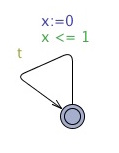
\includegraphics[width=2cm]{./images/tr1.jpg} &   %\hspace{1cm}
 %  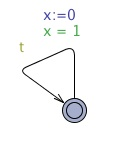
\includegraphics[width=2cm]{./images/tr2.jpg}
 \uppbox[20mm]{LEQ}{./images/tr1} &   %\hspace{1cm}
  \uppbox[20mm]{EQ}{./images/tr2}
\end{tabular}
\\[2mm]
are not \structure{timed-language equivalent}
% \\[2mm]
% \visible<2>{$\pair{(0,t)}$ is not a trace of the TLTS generated by the second system.}

}}
\end{columns}
\end{slide}

%----------------------------------------------------------------------------------
\begin{slide}{Bisimulation}
\small

\begin{block}{Timed bisimulation (between states of timed LTS)}
A relation $R$ is a \structure{timed simulation} iff whenever $s_1 R s_2$, for any action $a$ and delay $d$,
\begin{align*}
s_1\tran{a} s_1'\; & \imp\; \text{there is a transition}\; \; \; s_2 \tran{a} s_2' \land s_1' R s_2'\\
s_1 \tran{d} s_1'\; & \imp\; \text{there is a transition}\; \; \; s_2 \tran{d} s_2' \land s_1' R s_2'
\end{align*}
And a \structure{timed bisimulation} if its converse is also a timed simulation.
\end{block}
\end{slide}

%----------------------------------------------------------------------------------
\begin{slide}{Bisimulation}
\small

\begin{exampleblock}{Example}
\centering
% \wrap{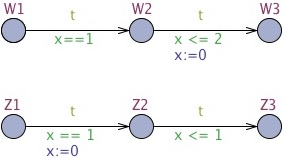
\includegraphics[width=6cm]{./images/bis1.jpg}}
\wrap{\uppbox[50mm]{W1-Z1}{./images/bis1.jpg}}
~~~~
\wrap{W1 bisimilar to Z1?}
\end{exampleblock}

\visible<2>{
\vspace*{-6mm}
\begin{align*}
\pair{\pair{W1,\{x\mapsto 0\}}, \pair{Z1,\{x\mapsto 0\}} } \in R
\end{align*}
where
\[\begin{array}{rlll}
R \; =\;  & \{\pair{\pair{W1,\{x\mapsto d\}}&, \pair{Z1,\{x\mapsto d\}} } &|~d \in \R_0^+\}\; \;   \cup\\
              & \{\pair{\pair{W2,\{x\mapsto d+1\}}&, \pair{Z2,\{x\mapsto d\}} } &|~ d \in \R_0^+\}\; \;  \cup\\
              & \{\pair{\pair{W3,\{x\mapsto d\}}&, \pair{Z3,\{x\mapsto e\}} } &|~d,e \in \R_0^+\}  
\end{array}\]
}


\end{slide}



%----------------------------------------------------------------------------------
\begin{slide}{Untimed Bisimulation}
\small

\begin{block}{Untimed bisimulation}
A relation $R$ is an \structure{untimed simulation} iff whenever $s_1 R s_2$, for any action $a$ and delay $t$,
\begin{align*}
s_1 \tran{a} s_1' \; & \imp\; \text{there is a transition}\; \; \; s_2 \tran{a} s_2' \land s_1' R s_2'\\
s_1 \tran{{\red{d}}} s_1'\; & \imp\; \text{there is a transition}\; \; \; s_2 \tran{{\red{d'}}} s_2' \land s_1' R s_2'
\end{align*}
And it is an \structure{untimed bisimulation} if its converse is also an untimed simulation.
\end{block}
~\\


\alert{Alternatively, it can be defined over a modified LTS in which all delays are abstracted on a 
unique, special transition labelled by $\epsilon$.}
\end{slide}

%----------------------------------------------------------------------------------
\begin{slide}{Untimed Bisimulation}
\small

\doExercise{W1 bisimilar to Z1?}{
\centering
\wrap{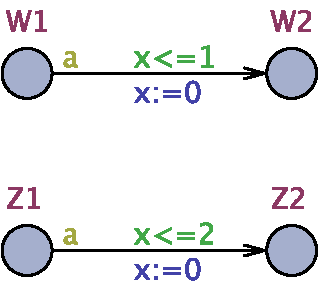
\includegraphics[height=3cm]{./images/bis2}}
% ~~~~
% \wrap{W1 bisimilar to Z1?}
}
\exerciseBack

\visible<2>{
\begin{align*}
\pair{\pair{W1,\{x\mapsto 0\}}, \pair{Z1,\{x\mapsto 0\}} } \in R
\end{align*}
where
\[\begin{array}{r@{~}l@{~}l@{~}l}
R \; =\;  & \{\pair{\pair{W1,\{x\mapsto d\}}&, \pair{Z1,\{x\mapsto d'\}} } &|~0\leq d \leq 1 , 0 \leq d' \leq 2 \}\; \;   \cup\\
      & \ldots
              % & \{\pair{\pair{W1,\{x\mapsto d\}}&, \pair{Z1,\{x\mapsto d'\}} } &|~ d>1, d'>2\}\; \;  \cup\\
              % & \{\pair{\pair{W2,\{x\mapsto d\}}&, \pair{Z2,\{x\mapsto d'\}} } &|~d,d' \in \R_0^+\}  
\end{array}\]
}


\end{slide}
\exerciseAdd

\section{Behavioural Properties}
%----------------------------------------------------------------------------------
\begin{slide}{Properties: expression and satisfaction}
\small
\begin{block}{The satisfaction problem }
Given a \alert{timed automata} $ta$ and a \structure{property} $\phi$, show that
\begin{equation*}
\TL{ta} \models \phi
\end{equation*}
\end{block}
~\\

\pause
\begin{itemize}
\item in which logic language shall $\phi$ be specified?
\item how is $\models$ defined?
\end{itemize}
\end{slide}




%----------------------------------------------------------------------------------
\begin{slide}{Expressing properties: \textsc{Uppaal}}
\small

\begin{block}{\textsc{Uppaal} variant of \textsc{CTL}}
\begin{itemize}
\item \structure{state formulae}:  describes individual states in $\TL{ta}$
\item \structure{path formulae}: describes properties of paths in $\TL{ta}$
\end{itemize}
\end{block}

\end{slide}

%----------------------------------------------------------------------------------
\begin{slide}{Expressing properties: \textsc{Uppaal}}
\small

\begin{block}{State formulae}
\vspace*{-4mm}
\begin{align*}
% \Pi\; ::=\; & \Ac \Boxc\, \Psi\, \mid\, \Ac\Diamondc\, \Psi\, \mid\, \Ec \Boxc\, \Psi\, \mid\, \Ec \Diamondc\, \Psi\, \mid\, \Phi \leadsto  \Psi\
% % \tag{path}
% \\[2mm]
\Psi\; ::=\; & ta.\ell ~|~ g_c ~|~ {\transp{g_d}} ~|~ \texttt{deadlock} ~|~
  \texttt{not~}\Psi ~|~ \Psi \texttt{ or }\Psi ~|~ \Psi \texttt{ and }\Psi ~|~
  \Psi \texttt{ imply }\Psi
  % \tag{state}
\end{align*}

Any expression which can be evaluated to a boolean value for a state (typically involving the 
\alert{clock constraints} used for guards and invariants and similar constraints over integer variables):
\vspace*{-6mm}
\begin{center}
\texttt{x >= 8}, \texttt{i == 8 and x < 2}, ...
\end{center}
Additionally,
\begin{itemize}
\item \structure{$ta.\ell$} which tests \alert{current location}:  $(\ell, \eta) \models ta.\ell$ \\
provided $(\ell, \eta)$ is a state in $\TL{ta}$
\item \structure{$\texttt{deadlock}$}: $(\ell, \eta) \models \forall_{d \in \R_0^+} .\, \text{there is no transition from} \; \pair{\ell,\eta+d}$ 
\end{itemize}

\end{block}

\end{slide}



\begin{slide}{Exercises}
  \centering
  \uppbox[7cm]{Lamp}{./images/Lamp}

  \doExercise{Write a state formula}{
  \vspace*{-8mm}
  \begin{enumerate}
    \item The lamp is \texttt{low}
    \item Not \texttt{off} and $y>25$
    \item If it is \texttt{low} or \texttt{bright}, then $y\leq 3600$
  \end{enumerate}
  }
  
\end{slide}

%----------------------------------------------------------------------------------
\begin{slide}{Expressing properties: \textsc{Uppaal}}
\small

\newcommand{\Boxc}{\alert{\Box}}
\newcommand{\Diamondc}{\alert{\Diamond}}
\newcommand{\Ac}{\structure{A}}
\newcommand{\Ec}{\structure{E}}

\begin{block}{Path formulae}
\begin{align*}
\Pi\; ::=\; & \Ac \Boxc\, \Psi\, \mid\, \Ac\Diamondc\, \Psi\, \mid\, \Ec \Boxc\, \Psi\, \mid\, \Ec \Diamondc\, \Psi\, \mid\, \Phi \leadsto  \Psi\
% \tag{path}
% \\[2mm]
% \Psi\; ::=\; & ta.\ell ~|~ g_c ~|~ {\transp{g_d}} ~|~ \texttt{deadlock} ~|~
%   \texttt{not~}\Psi ~|~ \Psi \texttt{ or }\Psi ~|~ \Psi \texttt{ and }\Psi ~|~
%   \Psi \texttt{ imply }\Psi
%   \tag{state}
\end{align*}

where
\begin{itemize}
\item \structure{$A$, $E$} quantify (universally and existentially, resp.) over \structure{paths}
\item \alert{$\Box$, $\Diamond$} quantify (universally and existentially, resp.) over \alert{states in a path}
\end{itemize}
also notice that

\vspace*{-3mm}
\begin{align*}
 \Phi \leadsto  \Psi\; \abv\; \Ac \Boxc\, (\Phi \imp \Ac \Diamondc\, \Psi)
\end{align*}
\end{block}

\end{slide}




% \uppbox[2.8cm]{\Large $A \Box\, \varphi$}{./images/AA.jpg}~~
% \uppbox[2.8cm]{$A \Diamond \, \varphi$}{./images/AE.jpg}


\begin{slide}{Expressing properties: \textsc{Uppaal}}
\small \centering

\uppbox[2.8cm]{\Large $A \Box\, \varphi$}{./images/AA.jpg}~
\uppbox[2.8cm]{\Large $A \Diamond \, \varphi$}{./images/AE.jpg}~~~~~
\uppbox[2.8cm]{\Large $E \Box\, \varphi$}{./images/EA.jpg}~
\uppbox[2.8cm]{\Large $E \Diamond\, \varphi$}{./images/EE.jpg}

\end{slide}

%----------------------------------------------------------------------------------
% \begin{slide}{Expressing properties: \textsc{Uppaal}}
% \small \centering

% ~\\
% \begin{tabular}{cc}
%   \Large $A \Box\, \varphi$ & \Large $A \Diamond \, \varphi$ \\
%  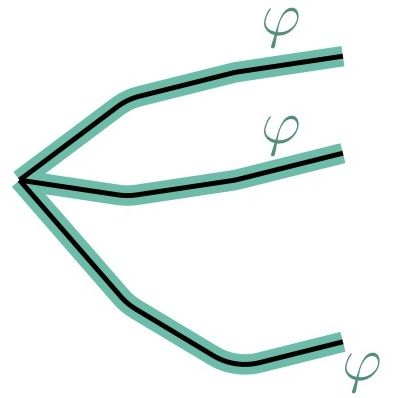
\includegraphics[width=2.8cm]{./images/AA.jpg} &
%  \hspace{1cm} 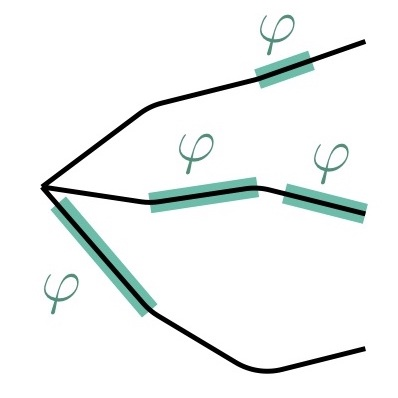
\includegraphics[width=2.8cm]{./images/AE.jpg}
% \end{tabular}

% ~\\[2mm]

% % \begin{block}{$E \Box\, \varphi$ and $E \Diamond\, \varphi$}
% \begin{tabular}{cc}
%   \Large $E \Box\, \varphi$ & \Large $E \Diamond\, \varphi$ \\
%  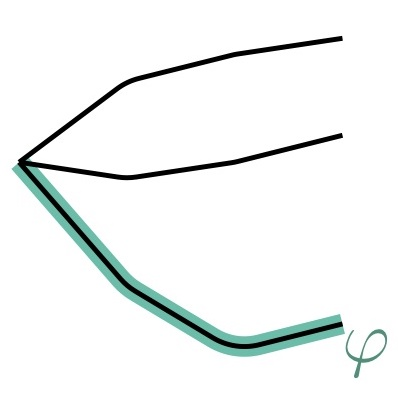
\includegraphics[width=2.8cm]{./images/EA.jpg} &   \hspace{1cm} 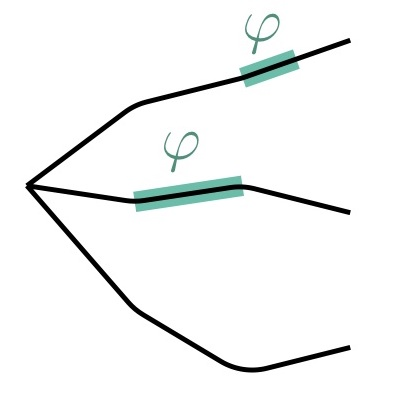
\includegraphics[width=2.8cm]{./images/EE.jpg}
% \end{tabular}
% % \end{block}
% \end{slide}

%----------------------------------------------------------------------------------
\begin{slide}{Expressing properties: \textsc{Uppaal}}
\small \centering

\uppbox[5cm]{\Large $\varphi\, \leadsto\, \psi$}{./images/LeadsTo.jpg}

% \begin{block}{$\varphi\, \leadsto\, \psi$}
% \begin{center}
%   \Large $\varphi\, \leadsto\, \psi$ \\
%  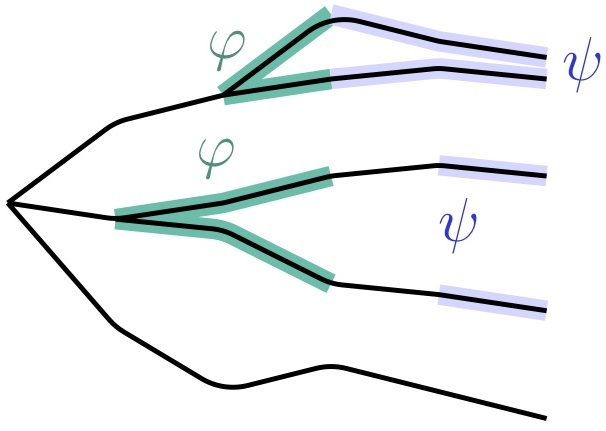
\includegraphics[width=5cm]{./images/LeadsTo.jpg} 
%  \end{center}
% \end{block}

\begin{exampleblock}{Example}
  If a message is sent, it will eventually be received -- $\texttt{send(m)} \leadsto \texttt{received(m)}$
\end{exampleblock}

\end{slide}

%----------------------------------------------------------------------------------
\begin{slide}{Reachability properties}
\small

\begin{block}{$E \Diamond\, \phi$}
\structure{Is there a path starting at the initial state, such that a state formula $\phi$ is eventually satisfied?}

\begin{itemize}
\item  Often used to perform sanity checks  on a model:
\begin{itemize}
\item \alert{is it possible for a sender to send a message?}
 \item \alert{can a message possibly be received?}
 \item ...
 \end{itemize}
 \item  Do not by themselves guarantee the correctness of the protocol (i.e. \alert{that any message is eventually delivered}), 
but they validate the basic behavior of the model.
 \end{itemize}
\end{block}

\end{slide}


%----------------------------------------------------------------------------------
\begin{slide}{Safety properties}
\small

\begin{block}{$A \Box\, \phi$ and $E \Box\, \phi$}
\vspace{5mm}
\structure{Something bad will never happen}\\
 or \structure{something bad will possibly never happen}
\vspace{5mm}

Examples\\
\begin{itemize}
\item \alert{In a nuclear power plant the temperature of the core is always (invariantly) under a certain threshold}.
\item \alert{In a game a safe state is one in which we can still win, ie, will possibly not loose}.
\end{itemize}

In Uppaal these properties are formulated positively: something good is invariantly true.
\end{block}

\end{slide}

%----------------------------------------------------------------------------------
\begin{slide}{Liveness properties}
\small

\begin{block}{$A \Diamond\, \phi$ and $\phi\, \leadsto \, \psi$}
\vspace{5mm}
\structure{Something good will \emph{eventually happen}}\\
 or \structure{if \emph{something} happens, then \emph{something else} will eventually happen!}
\vspace{5mm}

Examples\\
\begin{itemize}
\item \alert{When pressing the on button, then eventually the television should turn on}.
\item \alert{In a communication protocol, any message that has been sent should eventually be received}.
\end{itemize}

\end{block}

\end{slide}



%\end{document}




\begin{slide}{Exercise: worker, hammer, nail - revisited}
\small
\begin{columns}
\col[.45]{
  \centering
  ~\\[2mm]
  % Requires \usepackage{graphicx}
  % ~~~~\includegraphics[width=45mm]{./images/WHN.jpg}
  \uppbox[30mm]{Worker}{./images/Worker.pdf}\\[2mm]
  \uppbox[30mm]{Hammer}{./images/Hammer.pdf}\\[2mm]
  \uppbox[30mm]{Nail}{./images/Nail.pdf}\\
}
\col[.54]{
  \doExercise{Write properties and explain them}{
    \vspace*{-4mm}
    \begin{enumerate}
      \item Using $E\Diamond$
      \item Using $E\Box$
      \item Using $A\Diamond$
      \item Using $A\Box$
      \item Using $\leadsto$
    \end{enumerate}
    (Practice in UPPAAL)
  }
}
\end{columns}
\end{slide}


\begin{slide}{Exercise: write formulas}
  \centering
  \uppbox[4.5cm]{Lamp}{./images/Lamp}

  \vspace*{-2mm}
  \doExercise{Write formulas, and say which ones are true}{
    \vspace*{-8mm}
    % \begin{multicols}{2}
    \begin{enumerate}
      \item The lamp can become bright;
      \item The lamp will eventually become bright;
      \item The lamp can never be on for more than 3600s;
      \item It is possible to never turn on the lamp;
      \item Whenever the light is bright, the clock $y$ is non-zero;
      \item Whenever the light is bright, it will eventually become off.
    \end{enumerate}
    % \end{multicols}
    }
\end{slide}



\section{Examples: proving mutual exclusion}
% \section{Case-study: proving mutual exclusion}



%----------------------------------------------------------------------------------
\begin{slide}{The train gate example (1/2)}
\small

\begin{columns}

\col[0.35]{
\begin{center}
% \includegraphics[width=4cm]{./images/tg1.jpg}
\uppbox[5cm]{Train(id)}{./images/Train} 
\end{center}
}

\col[0.65]{
\begin{itemize}
\item \visible<2>{\texttt{E<> Train(0).Cross}}
\\ \structure{(Train 0 can reach the cross)}
\item \visible<2>{\texttt{E<> Train(0).Cross and Train(1).Stop}}
\\ \structure{(Train 0 can be crossing bridge while Train 1 is waiting to cross)}
\item \visible<2>{\texttt{E<> Train(0).Cross and}
\\ \texttt{~~~~~~~(forall (i:id-t)}
\\ \texttt{~~~~~~~~~~~~i != 0 imply Train(i).Stop)}}
\\ \structure{(Train 0 can cross bridge while the other trains are waiting to cross)}
\end{itemize}
}

\end{columns}
\end{slide}

%----------------------------------------------------------------------------------
\begin{slide}{The train gate example (2/2)}
\small

\begin{columns}

\col[0.35]{
\begin{center}
% \includegraphics[width=4cm]{./images/tg1.jpg}
\uppbox[5cm]{Train(id)}{./images/Train} 
\end{center}
}

\col[0.65]{
\begin{itemize}
\item \visible<2>{\texttt{A[] Gate.list[N] == 0}}
\\ \structure{There can never be N elements in the queue}
\item \visible<2>{\texttt{A[] forall (i:id-t) forall (j:id-t) Train(i).Cross \&\& Train(j).Cross imply i == j}}
\\ \structure{There is never more than one train crossing the bridge}
\item \visible<2>{\texttt{Train(1).Appr --> Train(1).Cross}}
\\ \structure{Whenever a train approaches the bridge, it will eventually cross}
\item \visible<2>{\texttt{A[] not deadlock}}
\\ \structure{The system is deadlock-free}
\end{itemize}
}
\end{columns}

\end{slide}



%%----------------------------------------------------------------------------------
%\begin{slide}{The train gate example}
%\small
%
%\begin{center}
%\includegraphics[width=5cm]{./images/tg2.jpg} 
%\end{center}
%
%\begin{itemize}
%\item Note the use of parameters and the select clause on transitions
%\item Programming ...
%\end{itemize}
%
%\end{slide}





%%----------------------------------------------------------------------------------
%\begin{slide}{Demo}
%\small
%
%
%\begin{itemize}
%\item The \alert{train gate} case study (included in the \textsc{Uppaal} distribution).
%\end{itemize}
%
%\end{slide}
%
%


%----------------------------------------------------------------------------------
\begin{slide}{Mutual exclusion}
\small

\begin{block}{Properties}
\begin{itemize}
\item \structure{mutual exclusion}: \alert{no two processes are in their critical sections at the same time}
\item \structure{deadlock freedom}: \alert{if some process is trying to access its critical section, then 
eventually some process (not necessarily the same) will be in its critical section; similarly for exiting the critical section}
\end{itemize}
\end{block}
\end{slide}

%%----------------------------------------------------------------------------------
\begin{slide}{Mutual exclusion}
\small


\begin{block}{The Problem}
\begin{itemize}
\item 
Dijkstra's original asynchronous algorithm (1965) requires, for $n$ processes to be controlled,
$\mathcal{O}(n)$ read-write registers and $\mathcal{O}(n)$ operations.
\item
This result is a theoretical limit (proved by Lynch and Shavit in 1992) which compromises scalability.
\end{itemize}
\end{block}
\pause
\fbox{but it can be overcome by introducing specific \structure{timing constraints}}
%\end{block}

\begin{block}{Two \emph{timed} algorithms:}
\begin{itemize}
\item  \structure{Fisher's protocol} (included in the \textsc{Uppaal} distribution)
\item  \structure{Lamport's protocol}
\end{itemize}
\end{block}
\end{slide}


%----------------------------------------------------------------------------------
\begin{slide}{Fisher's algorithm}
\small

\begin{block}{The algorithm}
\begin{align*}
\mathsf{repeat} & \\
& \mathsf{repeat}  \\
&  \hspace{1cm} \mathsf{await} \; id = 0\\
& \hspace{1cm} id := i\\
& \hspace{1cm}  \mathsf{delay}(k)\\ 
& \mathsf{until}\; id=i  \\
& \text{\emph{(critical section)}}\\
& id := 0\\
\mathsf{forever} &
\end{align*}
\end{block}
\end{slide}


%%----------------------------------------------------------------------------------
%\begin{slide}{Alur \& Taubenfeld's algorithm}
%\small
%
%\begin{block}{The algorithm}
%\begin{align*}
%\mathsf{repeat} & \\
%& s:\;  x:=i\\
%&\mathsf{await}\, (y = 0)\\
%& y := i\\
%& \mathsf{if}\;  x \neq i \; \mathsf{then}\,\\
%&  \hspace{1cm} \mathsf{delay}(2d); \\
%&  \hspace{1cm}  \mathsf{if}\; y \neq i \; \mathsf{then}\,\mathsf{goto}\, s; \\
%&  \hspace{1cm}  \mathsf{await}\, (\neg z)\\
%&  \mathsf{else}\, z:= true;\\
%& \text{\emph{(critical section)}}\\
%& z := false\\
%& \mathsf{if}\;  y = i \; \mathsf{then}\; y:=0;\\
%\mathsf{forever} &
%\end{align*}
%\end{block}
%\end{slide}


%----------------------------------------------------------------------------------
\begin{slide}{Fisher's algorithm}
\small
\begin{block}{Comments}
\begin{itemize}
\item One shared read/write register (the variable $id$)
\item Behaviour depends crucially on the value for $k$ --- the \structure{time delay}
\item Constant $k$ should be \alert{larger than the longest time that a process may take to perform a step while trying to get access to its critical section} 
\item This choice guarantees that whenever process $i$ finds $id = i$ on testing the loop guard it can enter safely ist critical section: \alert{all} other processes are out of the loop or with their index in $id$ overwritten by $i$.
\end{itemize}
\end{block}
\end{slide}

%----------------------------------------------------------------------------------
\begin{slide}{Fisher's algorithm in \textsc{Uppaal}}
\small
\centering

% 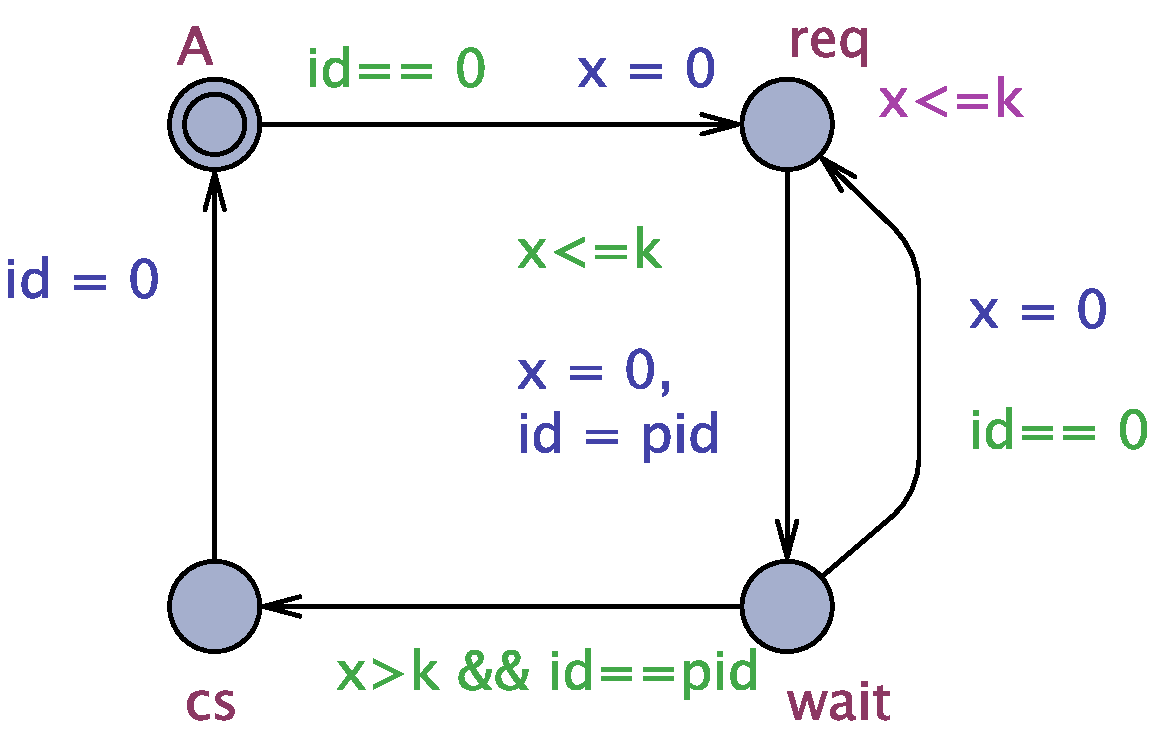
\includegraphics[width=6cm]{./images/P.pdf} 
\uppbox[5cm]{Fisher}{./images/P.pdf} 
%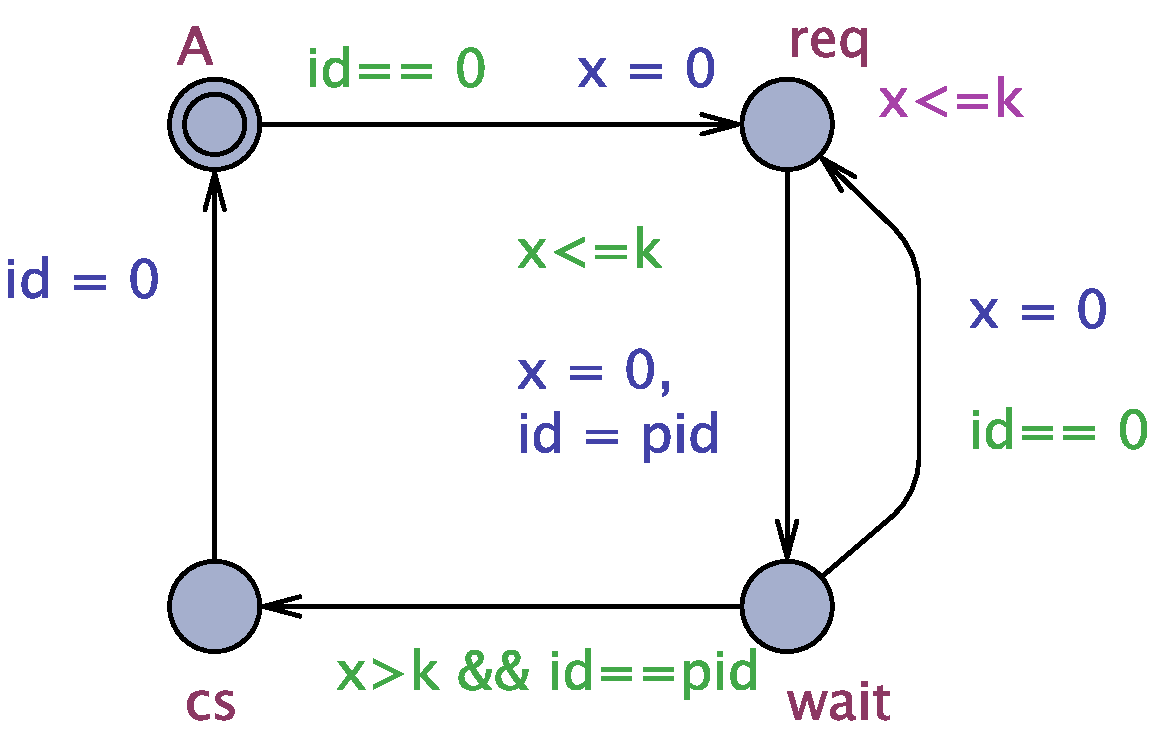
\includegraphics[width=1.1\textwidth]{./images/P.pdf} 


\begin{itemize}
\item Each process uses a local clock $x$ to guarantee that the upper bound between between its successive steps, while
trying to access the critical section, is $k$ (cf. \alert{invariant} in state $req$).
\item \alert{Invariant} in state $req$ establishes $k$ as such an upper bound
\item \alert{Guard} in transition from $wait$ to $cs$ ensures the correct delay before entering the critical section
\end{itemize}
\end{slide}

%----------------------------------------------------------------------------------
\begin{frame}[fragile]{Fisher's algorithm in \textsc{Uppaal}}
\small

\begin{block}{Properties}
%\includegraphics[width=12cm]{./images/ficher2.jpg} 
\begin{lstlisting}[emph={[2]forall,not}]
% P(1) requests access => it will eventually wait
P(1).req -> P(1).wait
% the algorithm is deadlock-free
A[] not deadlock
% mutual exclusion invariant
A[] forall (i:int[1,6]) forall (j:int[1,6])
   P(i).cs && P(j).cs imply i == j  
\end{lstlisting}
\end{block}

\begin{itemize}
\item The algorithm is \alert{deadlock-free}
\item It ensures  mutual exclusion if the correct timing constraints. 
\item ... but it is critically sensible to  small violations of such constraints: for example, replacing $x > k$ by 
$x \geq k$ in the transition leading to $cs$ compromises both \alert{mutual exclusion} and \alert{liveness}.
\end{itemize}
\end{frame}


%----------------------------------------------------------------------------------
\begin{slide}{Lamport's algorithm}
\small

\begin{block}{The algorithm}
\begin{align*}
\mathsf{start}: \; \;  &  a := i\\
& \mathsf{if}\; b \neq 0\; \mathsf{then\; goto\; start}\\
& b := i \\
& \mathsf{if}\; a \neq i\; \mathsf{then\; delay}(k)\\
& \hspace{12mm} \mathsf{else} \; \mathsf{if}\; b \neq i\; \mathsf{then\; goto\; start}\\
& \text{\emph{(critical section)}}\\
& b := 0
\end{align*}
\end{block}
\end{slide}

%----------------------------------------------------------------------------------
\begin{slide}{Lamport's algorithm}
\small
\begin{block}{Comments}
\begin{itemize}
\item Two shared read/write registers (variables $a$ and $b$)
\item Avoids \alert{forced waiting} when no other processes are requiring access to their critical sections
\end{itemize}
\end{block}
\end{slide}


%----------------------------------------------------------------------------------
\begin{slide}{Lamport's algorithm in \textsc{Uppaal}}
\small
\centering

% \begin{center}
% 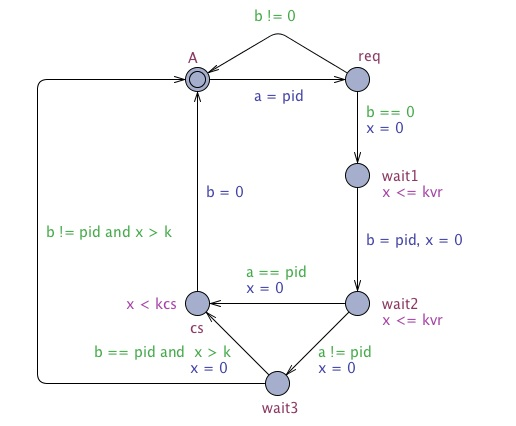
\includegraphics[width=9cm]{./images/lamport.jpg} 
\uppbox[80mm]{Lamport(pid)}{./images/lamport.jpg} 
% \end{center}

~\\[-6mm]

\hspace*{-130mm}%
\begin{tikzpicture}[remember picture, overlay]
  \node[draw=red,circle,very thick] at (242pt,125pt){~~~~};
  \node[draw=red,circle,very thick] at (242pt,69pt){~~~~};
  \node[draw=red,circle,very thick] at (159pt,51pt){~~~~};
  \node[draw=red,circle,very thick] at (128pt,76pt){~~~~};
  \node[draw=red,circle,very thick] at (132pt,107pt){~~~~};
\end{tikzpicture}

\end{slide}


%----------------------------------------------------------------------------------
\begin{slide}{Lamport's algorithm}
\small
\begin{columns}[T]

\col[0.43]{
\begin{block}{Model time constants:}
\begin{itemize}
\item \structure{$k$} --- time delay
\item \structure{$kvr$} --- max bound for register access
\item \structure{$kcs$} --- max bound for permanence in critical section 
\end{itemize}
Typically
\vspace{-10mm}
\begin{center}
\fbox{$k\; \geq \; kvr + kcs$}
\end{center}
\end{block}
}


\col[0.55]{
\begin{block}{Experiments}
\centering
\begin{tabular}{|l|c|c|c|c|}
\hline
& $k$ & $kvr$ & $kcs$ & verified? \\
\hline
Mutual Exclusion & 4 & 1 & 1 & Yes\\
Mutual Exclusion & 2 & 1 & 1 & Yes\\
Mutual Exclusion & 1 & 1 & 1 & No\\
No deadlock & 4 & 1 & 1 & Yes\\
No deadlock & 2 & 1 & 1 & Yes\\
No deadlock  & 1 & 1 & 1 & Yes\\
\hline
\end{tabular}
\end{block}
}
\end{columns}
\end{slide}


\end{document}
